\begin{evenBlock}{Clocks (10 min)}

\begin{minipage}[t]{\linewidth}
    \centering
    
    \begin{minipage}{.3\linewidth} % Left column and width
        \centering
        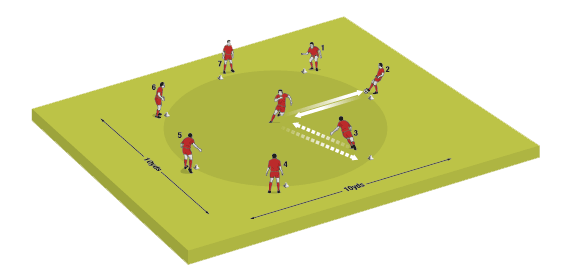
\includegraphics[width=\textwidth]{../img/Trimmed/Clocks1}
        \vspace{12pt}
        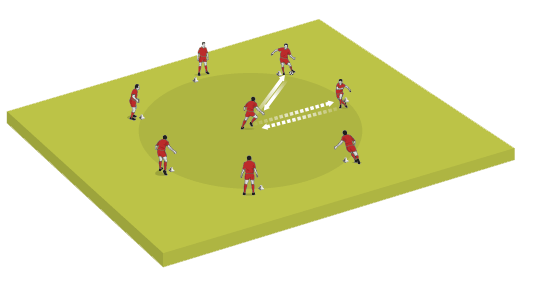
\includegraphics[width=\textwidth]{../img/Trimmed/Clocks2}
    \end{minipage}
    \hspace{0.05\linewidth}
    \begin{minipage}{.6\linewidth} % Left column and width
        \textbf{Drill Description:}
        Create a circle with your players of around 10 yards in diameter. Place cones around the circle where each player should stand, or go inside the centre circle and get the players to take a few steps forwards to get the right size. We’ve used eight players.
        \begin{enumerate}
        \setlength{\itemsep}{0pt}
        \setlength{\parskip}{0pt}
        \setlength{\parsep}{0pt}
        \item Start with the player in the middle who passes to one of the players around the circle
        \item Immediately the pass gets away, the centre player swaps position with the player clockwise from the player he passed to.
        \item The player he swaps with must get quickly into the centre to receive the ball and pass it to the next player anti-clockwise around the circle.
        \item Players continue to pass anti-clockwise and swap position with the player clockwise5. Try and get players to use one touch to get the ball around the clock
        \end{enumerate}
        
        \textbf{Coaching Points:}
        \begin{itemize}
        \setlength{\itemsep}{0pt}
        \setlength{\parskip}{0pt}
        \setlength{\parsep}{0pt}
        \item Focus on who gets your pass and then where you need to move.
        \item Attempt to complete this drill using a single touch.
        \end{itemize}

    \end{minipage}
\end{minipage}

\end{evenBlock}